\documentclass[12pt, fullpage,letterpaper]{article}

\usepackage[margin=1in]{geometry}
\usepackage{url}
\usepackage{amsmath,amsthm,amssymb}
\usepackage{float}
\usepackage{pgfplots}
\usepgfplotslibrary{polar}
\usepgflibrary{shapes.geometric}
\usetikzlibrary{calc}

\pgfplotsset{my style/.append style={axis x line=middle, axis y line=
middle, xlabel={$x$}, ylabel={$y$}, axis equal }}

\newcommand{\semester}{Fall 2016}
\newcommand{\assignmentId}{4}
\newcommand{\releaseDate}{Oct 18, 2016}
\newcommand{\dueDate}{Nov 1, 2016}

\newcommand{\bx}{{\bf x}}
\newcommand{\bw}{{\bf w}}
\DeclareMathOperator{\sgn}{sgn}

\title{CS 5350/6350: Machine Learning \semester}
\author{Gopal Menon\\Homework \assignmentId}
\date{\today}

\begin{document}
\maketitle

\section{PAC learning}
\label{sec:pac-learning}
\begin{enumerate}

\item ~[20 points total] A factory assembles a product that consist of
  different parts. Suppose a robot was invented to recognize whether a
  product contains all the right parts. The rules of making products
  are very simple: 1) you are free to combine any of the parts as they
  are 2) you may also cut any of the parts into two distinct pieces
  before using them. You wonder how much effort a robot would need to
  figure out the what parts are used in the product.

\begin{itemize}
\item[(a)] [5 points] Suppose that a naive robot has to recognize
  products made using only rule 1. Given $N$ available parts and each
  product made out of these constitutes a distinct hypothesis. How
  large would the hypothesis space be? Brief explain your answer.
    
\item[(b)] [5 points] Suppose that an experienced worker follows both
  rules when making a product. How large is the hypothesis space now?
  Explain.

\item[(c)] [10 points] An experienced worker decides to train the
  naive robot to discern the makeup of a product by showing you the
  product samples he has assembled. There are 6 available parts. If
  the robot would like to learn any product at $0.01$ error with
  probability $99\%$, how many examples would the robot have to see?
\end{itemize}


\item ~[20 points, from Tom Mitchell's book] We have learned an
  expression for the number of training examples sufficient to ensure
  that every hypothesis will have true error no worse than $\epsilon$
  plus its observed training error $error_S(h)$. In particular, we
  used Hoeffding bounds to derive
\[
	m \geq  \frac{1}{2 \epsilon^2}(\ln(|H|) + \ln(1/\delta)).
\]
Derive an alternative expression for the number of training examples
sufficient to ensure that every hypothesis will have true error no
worse than $(1+\epsilon)error_S(h)$, where $0 \leq \epsilon \leq 1$. You can use general Chernoff bounds
to derive such a result.

{\bf Chernoff bounds:} Suppose $X_1, \cdots, X_m$ are the outcomes of $m$ independent coin flips (Bernoulli trials), where the probability of heads on any single trail is $Pr[X_i = 1] = p$ and the probability of tails is $Pr[X_i = 0] = 1 - p$. Define $S = X_1 + X_2 + \cdots + X_m$ to be the sum of these $m$ trials. The expected value of $S/m$ is $E[S/m] = p$. The Chernoff bounds govern the probabilty that $S/m$ will differ from $p$ by some factor $0 \leq \gamma \leq 1$.

\begin{equation}
    \begin{array}{rcl}
	Pr[S/m > (1 + \gamma) p ] \leq e^{{-mp\gamma^2}/3}\\
	Pr[S/m < (1 - \gamma) p ] \leq e^{{-mp\gamma^2}/2}
	\end{array}
\end{equation}

\end{enumerate}

%%% Local Variables:
%%% mode: latex
%%% TeX-master: "hw"
%%% End:


\section{VC Dimensions}
\label{sec:vc-dimension}
\begin{enumerate}
\item ~[10 points] Suppose you have a finite hypothesis space
  $\mathcal{C}$. Show that its VC dimension at most
  $\log_2|\mathcal{C}|$ (Hint: You also prove this by contradiction.)

The growth function $m_\mathcal{C}(N)$ for a hypothesis class $\mathcal{C}$ is defined as the maximum number of dichotomies than can be generated by $\mathcal{C}$ on any $N$ points. 

The VC dimension of $\mathcal{C}$,$d_{VC}(\mathcal{C})$, is the largest $N$ for which $m_\mathcal{C}(N)=2^N$. In other words, $d_{VC}(\mathcal{C})$ is the largest $N$ that can be split into all possible dichotomies by the hypothesis class $\mathcal{C}$.

Each hypothesis in the hypothesis class $\mathcal{C}$ can at the maximum generate a distinct dichotomy. That means, there could be a maximum of $\left | \mathcal{C} \right| $ dichotomies that can be generated by the hypothesis class $\mathcal{C}$.

This means that $d_{VC}(\mathcal{C})$ is the largest $N$ such that 

\begin{equation*}
\begin{aligned}
m_\mathcal{C}(N)=2^N &= \left | \mathcal{C} \right| \\
N \log_2 2 &= \log_2 \left | \mathcal{C} \right| \\
N &= \log_2|\mathcal{C}|
\end{aligned}
\end{equation*}

This means that the VC dimension at most $\log_2|\mathcal{C}|$

\item ~[10 points] Given some finite domain set, $\mathcal{X}$, and a
  number $k \leq |\mathcal{X}|$, figure out the VC-dimension of each
  of the following classes and prove your claims:

  \begin{enumerate}
  \item
    $\mathcal{H}_{=k}^{\mathcal{X}} = \{h \in \{0,1\}^\mathcal{X} :
    |\{x : h(x) = 1\} | = k \}$. That is , the set of all functions that
    assign the value 1 to exactly $k$ elements of $\mathcal{X}$.

$d_{VC}(\mathcal{H})$, the VC dimension of the hypothesis class $\mathcal{H}$, is defined as the largest $N$ for which $m_{\mathcal{H}}(N) = 2^N$. The definition of $m_{\mathcal{H}} $ is similar to the one given above.\\

For the case of maximum number of dichotomies, we can consider that each hypothesis in $\mathcal{H}$ creates a distinct dichotomy. To find $d_{VC}(\mathcal{H})$ corresponding to this case, since we know that at exactly $k$ elements are assigned a label $1$ and the remaining elements are assigned label $0$, for the case of the VC dimension, the maximum number of dichotomies must be a power of $2$. Consider a subset of elements of $\mathcal{X}$, where $k$ elements are assigned label $1$ and $y$ elements are assigned label $0$.

\begin{equation*}
\begin{aligned}
\left | \mathcal{H} \right | &= 2^{k + y}\\
\log_2 \left | \mathcal{H} \right | &= k+y\\
y &= \log_2 \left | \mathcal{H} \right | - k\\
\end{aligned}
\end{equation*}

Since $d_{VC}(\mathcal{H})$, the VC dimension of the hypothesis class $\mathcal{H}$, is defined as the largest $N$ for which $m_{\mathcal{H}}(N) = 2^N$

\begin{equation*}
\begin{aligned}
2^{d_{VC}(\mathcal{H})} &= 2^{k+y}\\
&= 2^{k+\log_2 \left | \mathcal{H} \right | - k}\\
&= 2^{log_2 \left | \mathcal{H} \right |}\\
\implies d_{VC}(\mathcal{H}) &= \log_2 \left | \mathcal{H} \right |
\end{aligned}
\end{equation*}

  \item  $\mathcal{H}_{\leq k}^{\mathcal{X}} = \{h \in
    \{0,1\}^\mathcal{X} : |\{x : h(x) = 1\} | \leq k \quad or \quad |\{x
      : h(x) = 0\} | \leq k\}$. That is , the set of all functions that
    assign the value 1 or 0 to at most $k$ elements of $\mathcal{X}$.

For the case of a set of $d_{VC}(\mathcal{H})$ elements in $\mathcal{X}$, the label will be $1$ for between $0$ and $k$ elements. If this happens, there will be correspondingly between $k$ and $0$ elements with label $0$. So the total number of dichotomies will be
$$
\sum_{i=0}^k {N \choose i}
$$
where N is the number of elements chosen from $\mathcal{X}$.

Let $d_{VC}(\mathcal{H}) = y$. This means that

\begin{equation*}
\begin{aligned}
2^y &= \sum_{i=0}^k {N \choose i}\\
\implies d_{VC}(\mathcal{H}) &= y\\
 &= \log_2 \sum_{i=0}^k {N \choose i}
\end{aligned}
\end{equation*}

  \end{enumerate}

\item ~[10 points] Suppose we have an instance space consisting of
  real numbers and a hypothesis space $\mathcal{H}$ consisting of {\em
    two} disjoint intervals, defined by $[a, b]$ and $[c, d]$. That
  is, a point $x \in \Re$ is labeled as positive if, and only if,
  either $a \leq x \leq b$ or $c \leq x \leq d$. Determine the VC
  dimension of $\mathcal{H}$?

Since the two intervals are disjoint, there are three regions in the instance space that are defined by the intervals:

\begin{enumerate}
\item before the first interval
\item inside the first interval
\item between the first and second intervals
\item inside the second interval
\item after the second interval
\end{enumerate}

So the maximum number of points that can possibly be split into all possible dichotomies is $5$. If the $5$ points can be split into all possible dichotomies then the dichotomy $\{1,0,1,0,1\}$ should be one of them (I am representing a positive label by $1$ and a negative label by $0$). However, this dichotomy is not possible since there are only two intervals where the label can be $1$ and the label $\{1,0,1,0,1\}$ requires three such intervals.

Consider $4$ points. These $4$ points can be split into the dichotomies $\{\{0,0,0,0\},\{0,0,0,1\},\\\{0,0,1,0\},\{0,0,1,1\},\{0,1,0,0\},\{0,1,0,1\},\{0,1,1,0\},\{0,1,1,1\},\{1,0,0,0\},\{1,0,0,1\},\\\{1,0,1,0\},\{1,0,1,1\},\{1,1,0,0\},\{1,1,0,1\},\{1,1,1,0\},\{1,1,1,1\}\}$. These are all possible dichotomies that can be generated used $4$ points and the hypothesis space $\mathcal{H}$.\\ 

So $d_{VC}(\mathcal{H}) = 4$.

\item ~[15 points] We have a learning problem where each example is a
  point in $\Re^2$. The concept class $H$ is defined as follows: A
  function $h \in H$ is specified by two parameters $a$ and $b$. An
  example ${\bf x} = \{x_1, x_2\}$ in $\Re^2$ is labeled as $+$ if and
  only if $x_1 + x_2 \geq a$ and $x_1 - x_2 \leq b$ and is labeled $-1$
  otherwise.

  For example, if we set $a = 0, b = 0$, the grey region in figure
  \ref{f1} is the region of ${\bf x} = \{x_1, x_2\}$ that has label
  $+1$.

  \begin{figure}[h!]
    \centering
    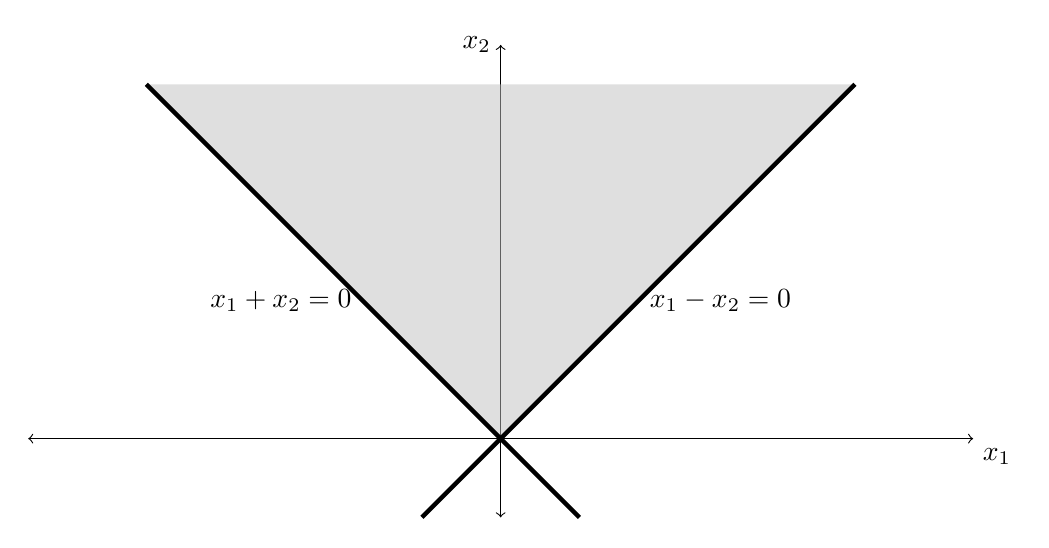
\begin{tikzpicture}[domain=0:2]
      \draw[<->] (-6,0) -- (6,0) node[below right] {$x_1$};
      \draw[<->] (0,-1) -- (0,5) node[left] {$x_2$};
      \fill[gray!50,opacity=0.5] (0,0) -- (4.5,4.5) -- (-4.5,4.5) -- (0,0);
      \draw [ultra thick] (4.5,4.5) -- node [midway,right] {$x_1 -x_2 = 0$} (-1,-1);
      \draw [ultra thick] (-4.5,4.5) --  node [midway,left] {$x_1 + x_2 = 0$}(1,-1);
    \end{tikzpicture}
    \caption{An example with $a = 0, b = 0$. All points in the gray region
      (extending infinitely) shows the region that will be labeled as
      positive.} \label{f1}
  \end{figure}



  What is the VC dimension of this class?

The concept class contains individual hypothesis' that consist on two arms that can intersect anywhere on $\Re^2$ and can cover an infinite arc from any angle from $0\si{\degree}$ to $360\si{\degree}$. This means that the concept class can split any $N$ points into all possible ($2^N$) dichotomies.\\

So $d_{VC}(H) = \infty$.

\item ~[{\bf For 6350 Students,} 15 points] Let two hypothesis classes
  $H_1$ and $H_2$ satisfy $H_1 \subseteq H_2$. Prove: $VC(H_1) \leq
  VC(H_2)$.

If $H_1 \subseteq H_2$, then any point marked with label $+1$ by a hypothesis in $H_1$ will be marked as $+1$ by a hypothesis in $H_2$ and any point marked with label $-1$ by a hypothesis in $H_1$ will be marked as $-1$ by a hypothesis in $H_2$.

Consider any set of points $N$ that are labelled by $H_2$. The same set of points may not result in the same number of dichotomies by $H_1$ as those produced by $H_2$. The reason is that $H_2$ may have hypotheses that are not present in $H_1$. This means that $H_2$ can be more expressive than $H_1$. This means that $d_{VC}(H_1) \leq d_{VC}(H_2)$.

\end{enumerate}
%%% Local Variables:
%%% mode: latex
%%% TeX-master: "hw"
%%% End:


\section{AdaBoost }

[15 points] You are given the following examples in the Table \ref{tab:AdaBoost}. You need to learning a model that minimize the error on this small dataset. 
\begin{table}[H]
  \centering
  \caption{training set}
  \label{tab:AdaBoost}
  \begin{tabular}{|c|c|}
    \hline
    ${\bf x} = [x_1,x_2]$  & y  \\ \hline
    [1,1]  & -1 \\ \hline
    [1,-1]  & 1 \\ \hline
    [-1,-1] & -1 \\ \hline
    [-1,1] & -1 \\ \hline
  \end{tabular}
\end{table}
Assuming you are also given the following 4 weak hypothesis classifiers
\begin{align*}
  h_a(\bf{x})&= \sgn(x_1) \\
  h_b(\bf{x}) &= \sgn(x_1-2) \\
  h_c(\bf{x}) &= -\sgn(x_1) \\
  h_d(\bf{x}) &= -\sgn(x_2) \\
\end{align*}
Treat them as your weak classifiers( rule of thumb) for the following
question.

Step through the full AdaBoost algorithm (Lecture Boosting slide P34)
for 4 rounds by choosing $h_t$ from the above 4 weak classifiers.
Remember that you need to {\bf choose a hypothesis } from $h_a, h_b,
h_c, h_d$ whose weighted classification error is {\bf better than
  chance}. However, in this question, for easier grading, we have
chosen $h_a$ as the first hypothesis and show the values of
$\epsilon_1$, $\alpha_1$, $Z_1$, $D_1$ in Table \ref{tab:Ada1}. 

For you answer, please follow the table template, report the
hypothesis you choose and all the $\epsilon_t$, $\alpha_t$, $Z_t$,
$D_t$, and the final hypothesis $H_{final}(x)$ for {\em four
  subsequent rounds}.
\begin{table}[H]
  \centering
  \caption{Choose $h_a({\bf x}) = \sgn(x_1), \epsilon_1 = 1/4, \alpha_1 = \frac{\ln3}{2} =0.5493, Z_1 = \frac{\sqrt{3}}{2}$}
  \label{tab:Ada1}
  \begin{tabular}{|c|c|c|c|c|c|}
    \hline
    ${\bf x} = [x_1,x_2]$ & $y_i$ & $h_a(x)$ & $D_1$ & $D_{1}(i)y_{i}h_t({\bf x_i})$ & $D_2$ \\ \hline
    [1,1]          &     -1  & 1    & 1/4   & -1/4                          &  3/6     \\ \hline
    [1,-1]         &    1   & 1    & 1/4   & 1/4                           &    1/6   \\ \hline
    [-1,-1]        &     -1  & -1    & 1/4   & 1/4                           & 1/6      \\ \hline
    [-1,1]         &     -1 & -1    & 1/4   & 1/4                           &  1/6     \\ \hline
  \end{tabular}
\end{table}

\begin{table}[H]
  \centering
  \caption{Choose $h_b({\bf x}) = \sgn(x_1 - 2), \epsilon_2 = 1/6, \alpha_2 = 0.8047, Z_2 = 0.7454$}
  \label{tab:Ada1}
  \begin{tabular}{|c|c|c|c|c|c|}
    \hline
    ${\bf x} = [x_1,x_2]$ & $y_i$ & $h_b(x)$ & $D_2$ & $D_{2}(i)y_{i}h_t({\bf x_i})$ & $D_3$ \\ \hline
    [1,1]          &     -1  & -1    & 3/6   & 3/6                          &  3/10     \\ \hline
    [1,-1]         &    1   & -1    & 1/6   & -1/6                          &    5/10   \\ \hline
    [-1,-1]        &     -1  & -1    & 1/6   & 1/6                           & 1/10      \\ \hline
    [-1,1]         &     -1 & -1    & 1/6   & 1/6                           &  1/10     \\ \hline
  \end{tabular}
\end{table}


\begin{table}[H]
  \centering
  \caption{Choose $h_c({\bf x}) = -\sgn(x_1), \epsilon_3 = 7/10, \alpha_3 = -0.4236, Z_3 = 0.9165$}
  \label{tab:Ada1}
  \begin{tabular}{|c|c|c|c|c|c|}
    \hline
    ${\bf x} = [x_1,x_2]$ & $y_i$ & $h_c(x)$ & $D_3$ & $D_{3}(i)y_{i}h_t({\bf x_i})$ & $D_4$ \\ \hline
    [1,1]          &     -1  & -1    & 3/10   & 3/10                          &  0.5000     \\ \hline
    [1,-1]         &    1   & -1    & 5/10   & -5/10                          &    0.3751   \\ \hline
    [-1,-1]        &     -1  & 1    & 1/10   & -1/10                           & 0.0714      \\ \hline
    [-1,1]         &     -1 & 1    & 1/10   & -1/10                           &  0.0714     \\ \hline
  \end{tabular}
\end{table}

The hypothesis $h_c(x)$ had an error worse than 0.5 and so was not used. The next iteration will use the same weights that were used in the third iteration.

\begin{table}[H]
  \centering
  \caption{Choose $h_d({\bf x}) = -\sgn(x_2), \epsilon_4 = 1/10, \alpha_4 = 1.0986, Z_4 = 0.6$}
  \label{tab:Ada1}
  \begin{tabular}{|c|c|c|c|c|c|}
    \hline
    ${\bf x} = [x_1,x_2]$ & $y_i$ & $h_d(x)$ & $D_4$ & $D_{4}(i)y_{i}h_t({\bf x_i})$ & $D_5$ \\ \hline
    [1,1]          &     -1  & -1    & 3/10   & 3/10                          &  0.1667     \\ \hline
    [1,-1]         &    1   & 1    & 5/10   & 5/10                          &    0.2778   \\ \hline
    [-1,-1]        &     -1  & 1    & 1/10   & -1/10                           & 0.5000      \\ \hline
    [-1,1]         &     -1 & -1    & 1/10   & 1/10                           &  0.0556     \\ \hline
  \end{tabular}
\end{table}

Final Hypothesis:
$H_{final}(x) = 0.5493 \times h_a(x) + 0.8047 \times h_b(x) + 1.0986 \times h_d(x)$


\begin{table}[H]
  \centering
  \caption{Apply Final Hypothesis on test data}
  \label{tab:Ada1}
  \begin{tabular}{|c|c|c|c|c|c|c|}
    \hline
    ${\bf x} = [x_1,x_2]$ & $y_i$ & $h_a(x)$ & $h_b(x)$ & $h_d(x)$ & $H_{final}(x)$ \\ \hline
    [1,1]          &     -1  & 1    & -1   & -1                         &  -1     \\ \hline
    [1,-1]         &    1   & 1    & -1   & 1                          &    1   \\ \hline
    [-1,-1]        &     -1  & -1    & -1   & 1                           & -1      \\ \hline
    [-1,1]         &     -1 & -1    & -1   & -1                           &  -1     \\ \hline
  \end{tabular}
\end{table}
%%% Local Variables:
%%% mode: latex
%%% TeX-master: "hw"
%%% End:



\end{document}
%%% Local Variables:
%%% mode: latex
%%% TeX-master: t
%%% End:
